\chapter{Motivation}
\label{ch:motivation}

\section{Current Research}

In the current research, we could see the usage of multiple tools in the Software Industry where each tool is different in computation approaches as one could be standard run on Nightly builds for example with Checkmarx \cite{checkmarx} tool or could be following Incremental Analysis, which means only testing the changed version of code instead of running analysis on complete codebase. The reasons of using multiple tools could be as each tool is capable of detecting bugs with different coverage \cite{bessey2010few} \cite{delaitre2015evaluating}, it could help in finding more bugs easily which are not found by tool but the other \cite{plakosh2014improving}. There is also research \cite{flynn2018prioritizing} going in the direction of using multiple static analysis tools in order to prioritise the bug warning alerts. There is a paper \cite{meng2008approach} published in 2008 which uses results of three different static analysis tools for a programming language, Java and merges them together in order to show warnings to the developer. Also, recently a team from OASIS \cite{oasis} in the OASIS SARIF Technical Committee \cite{oasis-tc} introduced a Static Analysis Results Interchange Format (SARIF) of representing bug warnings in a JSON format. Currently \cite{sarif-git}, the specification is being standardised. This shows there is potential research going in direction of using multiple static analysis tools at once. This shows the potential of using multiple tools in near future once the standardisation is adapted across static analysis tools developers or at least with the availability of adapters which are capable of converting the output of one static analysis tool to a SARIF format. Here's an example \cite{sarif-example} of how SARIF might look. SARIF is been used by SWAMP \cite{swamp-scarf-sarif}, a continuous software assurance which is automated.

\begin{lstlisting}[language=json,firstnumber=1][frame=single]

"results": [
{
"ruleId": "GSV001",
"message": {
"text": "Variable \"i\" was used without being initialized.",
"richText": "Variable `i` was used without being initialized." 
},
"locations": [
{
"physicalLocation": {
"uri": "file://build.example.com/work/src/collections/list.cpp", "region": {
"startLine": 16
}
},
"fullyQualifiedLogicalName": "collections::list:add"
}
]


\end{lstlisting}


Although we have seen the current research trends and their direction, the usability aspect is not addressed so far in the context of using multiple tools. There are no research papers found addressing the usability issue with multiple tools in single interface. The multiplicity of tools used for a single project and that too with different computation capabilities brings a new challenge.  One tool could produce results in no time and others could take more time in comparison. This could lead to a situation of breaking the usability of the user interface. On that challenge, this thesis aims to address such a scenario with a problem statement as " How to integrate the results of multiple static analysis tools in a unified user interface? ".  \\ \\

The thesis work begins by brainstorming on the problem statement and as a result, different research questions are brought up and of which three research questions are selected with respect to available sources, scope and limitations of Thesis time frame. \\ \\

\section{What Current Tools do?}

Let us now examine each research question and see what the current tools behave like. \\ \\

\textbf{1. How to display results for the same codebase from different analysis tools?}  \\

This question needs to address the scalability aspect of displaying results as usage of multiple tools results in redundancy and a high number of warnings with more coverage. The following figure \ref{fig:findbugs-results} shows how a FindBugs \cite{findbugs} static analysis tool shows results for a project \cite{findbugs-example}. This could be the same with other tool and so when you use multiple tools, there is a need for a better user interface.\\ \\

\begin{figure}[hbt!]
	\centering
	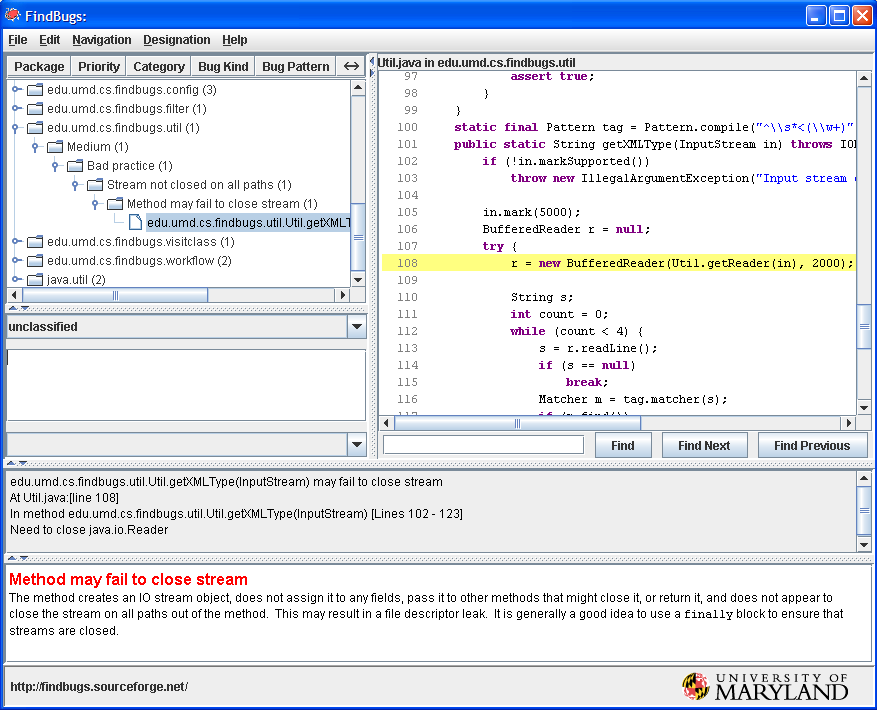
\includegraphics[width=\linewidth]{figures/findbugs-results}
	\caption{A preview of FindBugs scan results.}
	\label{fig:findbugs-results}
\end{figure}

\clearpage

\textbf{2. What feedback works to know that the bug fixing is on-going?} \\

This question needs to address the scenario where one tool could give an instant update on the bug fixing process and others might take more time to analyse and report the update on it. In the design aspect, especially the User Interface needs to be adaptive \cite{NB18} enough as static analysis tools sometimes take a long time to stop and there is no intuitive feedback provided. Also, One interesting aspect of Johnson et. al. \cite{JSMB13} study is about the importance of feedback from tools without disrupting the developer workflow. Traditionally, the project files are added to FindBugs \cite{findbugs} tool as seen in the figure \ref{fig:findbugs-scan} in order to start the scanning and the user has to wait for some minutes to see the results. There was no feedback in the process of scanning. \\ \\

\begin{figure}[hbt!]
	\centering
	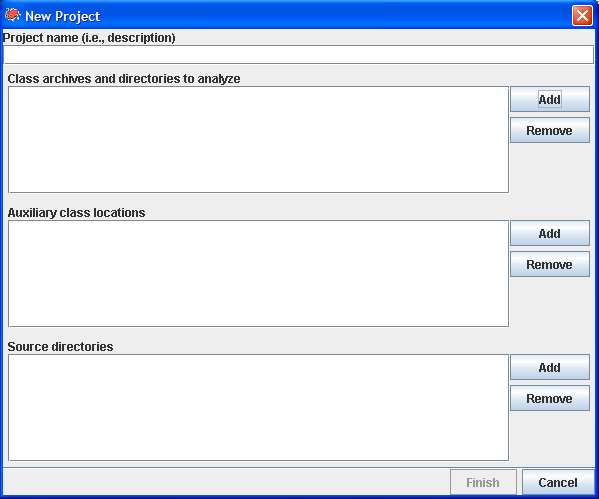
\includegraphics[width=\linewidth]{figures/findbugs-scan}
	\caption{A preview of initiating FindBugs to scan a project.}
	\label{fig:findbugs-scan}
\end{figure}

Back in the history of Computer Science, there is an observation made when the user interface is non-responsive, the user shuts down the system. Thereafter, comes to the implementation of user interface called Ghost screen by Colleran et al. \cite{colleran} who patented the method which manages application programs with non-responsive user interfaces in the year 2005. About the response times, NN Group \cite{nn} states that if the execution of a certain task takes 0.1 up to 1 second then there is no need for feedback, just show the result. If it takes 10 seconds, there should be feedback and if it is variable every time then there is the importance of per cent bar \cite{Borman} but sometimes it could be overkill to use as it cause stress to the user by the principle of display inertia. If the time taken by a task is unknown then there has to be feedback like a spinning ball or in an example of a task being to scan databases then it has to report user what database is being scanned currently. Overall, there has to be feedback stating that the system is working, if not indicating what is actually doing. This motivates to know how responsiveness in terms of usability is vital to consider in the development of modern tools. Further, this needs to be addressed in the context of using multiple tools.\\ \\


\textbf{3. How to carry traceability of bug fixing?} \\

In the scenario, where the user has picked a bug to fix and worked on it and later he submitted for analysis. Then the bug could either get fixed or new bugs could have been introduced or different bugs got resolved by fixing the one bug. All these might have taken place and this is uncertain. Thereby it would be better to have traceability in order to somehow safeguard the code repository from future bugs or monitor the changes happening in the context of bugs. \\ \\

As per the related work in research \cite{heinemann2014teamscale}, a tool named "Teamscale" \cite{teamscale} shows the influence on the quality status for each change in code backed by version control commits. For a change, it shows how many quality problems are added or removed. The illustration could be observed in the following figure \ref{fig:teamscale}.\\ \\

\begin{figure}[hbt!]
	\centering
	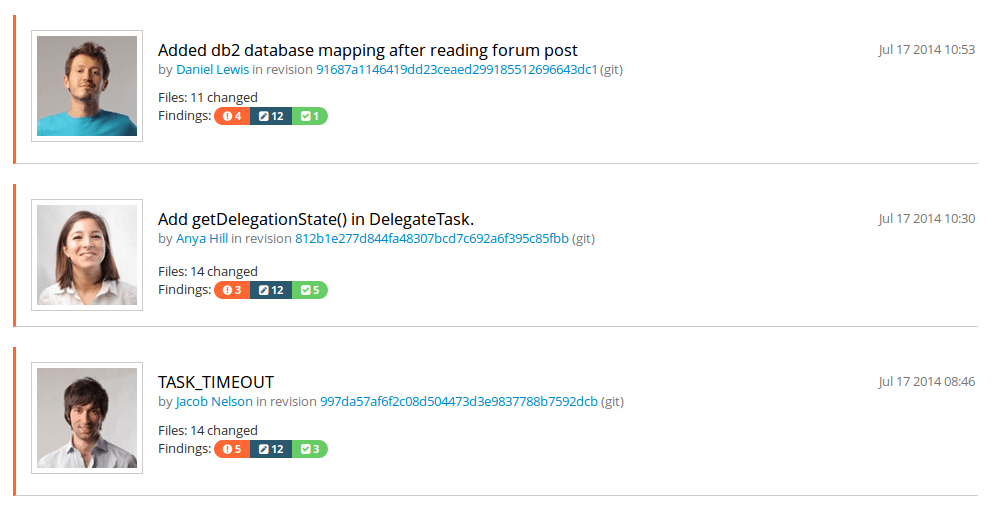
\includegraphics[width=\linewidth]{figures/teamscale}
	\caption{A Teamscale feature of showing quality status with code changes.}
	\label{fig:teamscale}
\end{figure}

\let\cleardoublepage\clearpage
